%-----------------------------------------------------------------------------%
\chapter{\babDua}
%-----------------------------------------------------------------------------%
Unit IT merupakan salah satu unit kerja di lingkungan UMS yang memiliki tugas utama untuk memberikan dukungan penyediaan layanan teknologi informasi terhadap semua aktivitas akademik maupun non akademik di lingkungan UMS.
%-----------------------------------------------------------------------------%
\section{Sejarah}
%-----------------------------------------------------------------------------%

Di UMS manajemen sistem informasi dikelola oleh unit Information Technology (IT) berkoordinasi dengan unit-unit lain yang ada di UMS. Unit IT-UMS secara organisatoris berada dibawah Wakil Rektor II.

Unit IT didukung oleh personal dengan kemampuan yang sesuai dengan bidang kerjanya, meskipun dalam jumlah yang terbatas. Manajer bidang sistem informasi diambil dari staff dosen Teknik Elektro yang berpengalaman dalam bidang computer network, database system dan programming. Ketua Bidang Program dan Basisdata berasal dari staff karyawan yang berpengalaman dalam bidang sistem basisdata. Bidang Pemeliharaan Web berasal dari staff dosen Teknik Elektro meskipun sudah cukup trampil dalam bidang pemrograman tapi untuk bidang pemeliharaan web masih perlu banyak belajar. Bidang Pemeliharaan jaringan juga berasal dari staff dosen Teknik Elektro, meskipun sudah berpengalaman dalam bidang jaringan komputer tetapi tingkat penguasaannya masih perlu ditingkatkan. Bidang Programmer berasal dari karyawan part-time berpengalaman dalam bidang pemrograman basisdata.

Pada dua tahun terakhir ini pimpinan UMS mulai memberikan perhatian khusus terhadap pengembangan sistem informasi agar mampu menyediakan data dan informasi secara cepat dan akurat. Meskipun keberadaan jaringan komputer internal (LAN) kampus sudah ada sejak Tahun 1990 namun pemanfaatannya belum efektif karena sampai dengan awal 2005 belum ada unit khusus yang bertugas memelihara jaringan serta belum ada kebijakan yang jelas terhadap masalah infrastruktur IT.

Melihat kondisi ini maka pada pertengahan 2005, di era kepemimpinan yang baru, UMS telah menugaskan unit IT dengan tugas untuk memelihara jaringan komputer kampus serta meningkatkan kualitas pelayanan sehingga dapat dijadikan sebagai basis sistem informasi yang memadahi untuk menjalankan manajemen pendidikan di UMS.  Unit IT ini diharapkan akan dapat dijadikan sebagai dasar bagi perkembangan TIK di UMS.

\section{Visi}
\begin{enumerate}[itemsep=-1ex]
\item Adanya sistem administrasi akademik yang terintegrasi yang memungkinkan UMS melakukan suatu sistem kontrol kualitas yang bertahap dari jurusan hingga ke tingkat universitas.
\item Memiliki sistem administrasi akademik yang terintegrasi terhadap aspek keuangan, kepegawaian, dan perpustakaan.
\end{enumerate}

\section{Misi}
\begin{enumerate}[itemsep=-1ex]
\item Mengembangkan dan memelihara sistem administrasi akademik, perpustakaan dan keuangan yang terintegrasi di seluruh UMS agar selalu up-to-date dan pada kondisi up and running.
\item Mengatur, mengontrol dan memelihara sistem internet beserta prosedur yang terkait dengan sistem administratif komputer.
Membina, melatih dan melakukan upgrade terhadap staff dosen dan administrator komputer sampai ke tingkat jurusan.
\item Mengatur, mengamankan, dan merawat database akademik serta database yang terkait.
\item Mengadakan kerjasama di bidang teknologi informasi, baik dengan provider maupun manufacture.
\end{enumerate}

\section{Rencana Pengembangan}
Untuk lima tahun ke depan dalam rangka mencapai target yang telah disebutkan di atas pimpinan UMS  telah mencanangkan hal-hal sebagai berikut :

\begin{enumerate}[itemsep=-1ex]
\item Peningkatan jangkauan dan kualitas layanan IT-UMS. Jangkauan dan kualitas layanan IT-UMS  ditingkatkan antara lain dengan meningkatkan kualitas sistem jaringan di dalam (LAN: Local Area  Network) dan di luar (WAN: Wide Area Network)  serta peningkatan kualitas SIM (Sistem    Informasi Manajemen).

\item Pembangunan sistem basisdata terintegrasi. Keberadaan sistem basis data yang handal merupakan syarat bagi terbangunnya SIM universitas yang handal. Sistem basisdata dibangun secara terpusat pada IT-UMS namun transaksi data harus terjadi pada tiap unit kerja dimana data bersumber. Dengan pola yang demikian, akan dapat dihindari proses input data yang berulang.

\item Peningkatan kualitas sumber daya manusia bidang TIK. Fasilitas TIK akan menjadi tidak bermanfaat jika para penggunanya tidak memiliki kemampuan yang memadai. Diperlukan adanya  pelatihan yang berkesinambungan bagi para staff dan karyawan UMS.
\end{enumerate}

\section{Struktur Organisasi}

\begin{figure}
\begin{center}
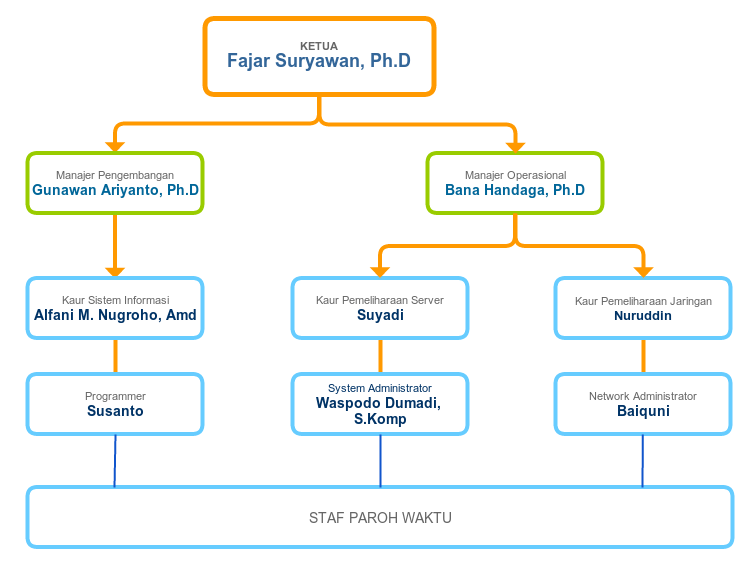
\includegraphics[width=1.0\textwidth]{pics/struktur.png}
\end{center}
\caption{Struktur Organisasi Unit IT UMS}
\end{figure}    

